% Drawing 161-6/02-4 -- folder 161-6, batch 02, archive page 21 (PDF page 22).
% Transcription: plus bas encore, un cercle avec un diamètre prolongé hors du cercle des deux côtés (vers le haut jusqu'au cercle précédent), une corde horizontale qui le coupe en un point marqué, et deux points marqués sur le bord, en haut ; à gauche, un arc intérieur descend du point marqué de gauche.
% Kind: circle with a prolonged diameter and marked points. Method 2 (schematic redraw from the facsimile). Status: ok.
% Notes: A circle (an ellipse fitted to his outline, slightly tilted); a straight stroke through it, prolonged beyond the circle at both ends (upwards to the figure above, downwards to a small dot), passing through a marked point of the outline at the upper right and a marked point inside (slightly off the centre, so the stroke is not exactly a diameter); a horizontal chord through that inner point, from outline to outline; a second marked point on the outline at the upper left, from which a nearly straight stroke runs down the left side to a marked point near the bottom; beside its top a short arc starting at a small dot; an arc sweeping from the left of the outline to below the centre, and a second marked point at its foot. Redrawn 2026-11-10 (issue 128). 2026-11-13, Claude Opus 5.5, issue 147, overlay check: not compiled (no TeX in the session); the TikZ was rasterised by a local interpreter and laid over the 299 ppi scan rendered at 400 dpi. Redrawn on the ink: the outline refitted as a tilted ellipse on its ink (it was about two units too low), the strokes fitted by least squares or through points moved onto their ink, the points on their blots; every stroke lies on its ink to within about one unit. Changed: the stroke down the left side is nearly straight, as on the page; the short arc beside it, its dot and the two marked points at the bottom left are added.
% Coordinates: 1 unit = 1 mm = 1/100 of the crop width (bbox in page fractions: [0.14, 0.395, 0.3, 0.48]).
% Redrawn by Claude (claude-fable-5-2), issue #128, 2026-11-10; not checked by a human; not compiled (no TeX in the session); overlay-checked on the scan by Claude Opus 5.5, issue #147, 2026-11-13, not compiled (no TeX in the session).
% Rights: reproduces part of the work -- behind RENDER_TRANSCRIPTS, never published by itself.
\documentclass[tikz,border=3pt]{standalone}
\usepackage{amsmath,amssymb}
\usetikzlibrary{patterns,arrows.meta}
\tikzset{pencil/.style={black!45}, struck/.style={black!35}, mpt/.style={circle,draw,inner sep=1.3pt}, pt/.style={circle,fill,inner sep=0.9pt}, opt/.style={circle,draw,fill=white,inner sep=1.1pt}}
\begin{document}
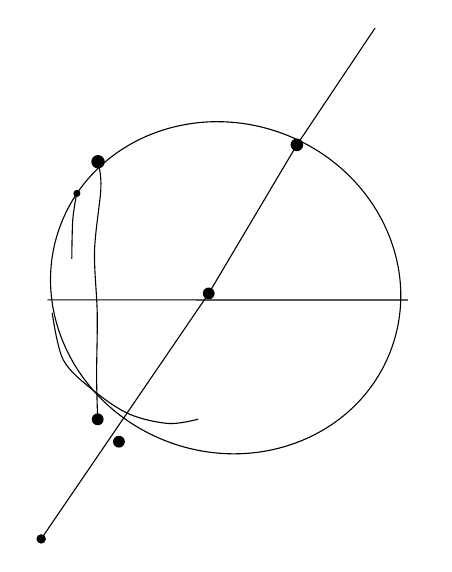
\begin{tikzpicture}[x=1mm,y=1mm,line cap=round,line join=round,font=\scriptsize]
\draw[rotate around={-21:(49.24,-34.73)}] (49.24,-34.73) ellipse[x radius=22.43, y radius=20.88];
% the prolonged diameter, through the upper right point of the outline and the inner point
\draw (68.2,-1.77) -- (58.29,-16.58) -- (47.09,-35.45) -- (25.81,-66.63);
\fill (58.29,-16.58) circle [radius=0.8];
\fill (47.09,-35.45) circle [radius=0.75];
\fill (33.03,-18.73) circle [radius=0.85];
\fill (25.81,-66.63) circle [radius=0.6];
\draw (26.64,-36.27) -- (72.36,-36.29);
% inner strokes at the left: a nearly straight stroke down from the upper left point, a short arc beside it, an arc sweeping from the left of the outline to below the centre
\draw plot[smooth, tension=0.55] coordinates {(33.03,-18.73) (33.4,-22) (32.59,-30) (32.93,-38) (32.85,-46) (32.99,-51.44)};
\draw plot[smooth, tension=0.55] coordinates {(30.36,-22.59) (29.83,-26.02) (29.7,-31)};
\fill (30.35,-22.75) circle [radius=0.45];
\draw plot[smooth, tension=0.55] coordinates {(27.22,-37.95) (28.64,-43.93) (32.53,-47.84) (37.01,-50.78) (41.98,-51.97) (45.72,-51.43)};
\fill (32.99,-51.44) circle [radius=0.75];
\fill (35.69,-54.28) circle [radius=0.75];
\end{tikzpicture}
\end{document}
